\documentclass[12pt]{report}
\usepackage[T1]{fontenc}
\usepackage{setspace}
\usepackage{lmodern}
\usepackage{colortbl}
\setlength{\parskip}{1ex plus 0.5ex minus 0.2ex}
\usepackage{color}
\usepackage{ucs}
\usepackage{placeins}
\usepackage[french]{babel}
\usepackage{datetime}
\usepackage{graphicx}
\usepackage{lscape}
\usepackage[toc,page]{appendix} 
\usepackage{listingsutf8}
\definecolor{grey}{rgb}{.9,0.9,0.9}
\setlength\voffset{0.3in}
\setlength\headheight{25pt}
\usepackage{url} 
\lstset{ % general style for listings 
   numbers=left 
   , tabsize=2 
   , frame=single 
   , breaklines=true 
   , basicstyle=\ttfamily 
   , numberstyle=\tiny\ttfamily 
   , framexleftmargin=13mm 
   , backgroundcolor=\color{grey} 
   , xleftmargin=12mm 
   , frameround={tttt} 
   , captionpos=b 
} 
\lstdefinestyle{xslt} 
{ 
    emph={xsl,template,variable,param,for,each,apply,templates,with,param} 
    , emphstyle=\color{magenta} 
    , emph={[2]match, select, name, mode} 
    , emphstyle={[2]\color{cyan}} 
}
\usepackage{multirow}
\usepackage{geometry}
%% We will completely define our own header strings, so switch the fancy
%% headers on, but nuke all the default values. (Note that this package
%% *has* to load after the geometry package!)

\usepackage{fancyhdr}
\renewcommand{\headrulewidth}{0pt}
\usepackage{lastpage}
\pagestyle{fancy}
\lfoot{Auteur: David Cormier (DC)}
\lhead{
    \begin{tabular}{| l | c | r | c | c |}
      \hline
      \multirow{2}{*}{Ecole de technologie superieure} & Cours: LOG792 & Document: 1 & Date: \today & Version 1\\ \cline{2-5}
& \multicolumn{2}{|r|}{Rapport d'etape} & \multicolumn{2}{|r|}{\pageref{LastPage} pages} \\
\hline
    \end{tabular}
}
\chead{}
\rhead{}
\usepackage[utf8x]{inputenc}
\usepackage{geometry}
\geometry{left=3cm, right=2cm, top=2cm}


\title{Rapport d'étape}
\author{David Cormier}
\begin{document}
\begin{titlepage}


\includegraphics[width=2cm]{./ets}
\begin{center}
\Large Rapport d'étape \\[1cm]
\Large Projet de fin d'études \\[0.5cm]
\Large Département de génie logiciel et des TI\\[1.0cm]
\hrule \\[0.2cm] 
\LARGE Identification des références bibliographiques dans un texte et acquisition du contenu référé par celles-ci\\[0.2cm]
\hrule \\[4cm]
David Cormier\\
CORD14068406\\[2cm]
Professeur superviseur\\
Christian Desrosiers\\[2cm]
Le 29 octobre 2011
\end{center}
\end{titlepage}


\tableofcontents
\newpage
\listoffigures
\listoftables
\newpage
\onehalfspacing
\setcounter{chapter}{1}
\section{Glossaire}
%\fontsize{4.5mm}{6.5mm}\selectfont
\begin{tabular}{| p{3cm} | p{12cm} |}
    \rowcolor[gray]{0.9} \hline
    Terme & Définition \\ \hline
    \emph{boxfile} & Document spécifiant, pour chacun des caractères numérisés par \emph{Tesseract}, la position et la dimension du carré à l'intérieur duquel le caractère a été identifié \\ \hline
    \emph{hOCR} & Fichier HTML utilisant des métadonnées pour décrire les attributs d'un document numérisé (positions et dimensions des lignes, nombre de colonnes, etc.) \\ \hline
    \emph{Tesseract} & Logiciel de reconnaissance de caractère développé par Hewlett-Packard dans les années 90 et maintenant développé en \emph{open source} sous la gouverne de Google. \\ \hline
    \emph{HTML} & \emph{HyperText Markup Language}, standard utilisé pour les pages WEB \\ \hline
    \emph{CSS} & \emph{Cascading Style Sheets}. Tandis que les fichiers HTML décrivent la structure du document, les fichiers CSS en décrivent le style.
\end{tabular}
\newpage


\section{Introduction}
De nombreux projets visent à numériser des références bibliographiques traditionnelles. Les références numériques ont ceci d'intéressant par rapport aux références traditionnelles qu'il est possible d'utiliser l'ordinateur pour faire des analyses sur un corpus dont la taille aurait rendu la tâche impossible autrement.

Les références numériques offrent aussi, en raison de leur format, une plus grande interactivité, car en plus de contenir le texte de la référence -- leur vocation première, elles peuvent aussi contenir, et ce de manière transparente pour l'utilisateur, un ensemble de métadonnées. Ces métadonnées peuvent alors servir de support sur lequel sont basées les fonctionnalités offertes par le document.

Dans ce texte, nous allons analyser les manières d'augmenter les références d'une ressource référence numérisée en faisant pointer les références textuelles vers l'endroit où réside le texte sur Internet. Nous allons dans un premier temps décrire la problématique propre à l'identification de références et à la localisation de celles-ci, pour ensuite décrire le travail qui sera accompli pour résoudre le problème. Après avoir décrit les objectifs, la méthode retenue pour accomplir le travail sera décrite et la description de la solution sera offerte.


\section{Problématique et contexte}
L'identification des sources et la recherche de références bibliographiques sont à la base de la recherche académique. Tout lecteur désirant approfondir les connaissances qu'il a de son domaine d'intérêt ira consulter les références bibliographiques des textes qu'il lit pour pouvoir obtenir les références connexes.

Les publications universitaires prennent essentiellement le même format, à quelques différences près selon la discipline. Cette standardisation du format leur permet de véhiculer le message plus efficacement en tirant profit de l'association cognitive qui se crée implicitement chez le lecteur entre le format du texte et sa fonction. 

Par exemple, le format de la citation varie très peu d'un article scientifique à l'autre et cette variation est dans la majorité des cas explicable par le standard particulier qui a été adopté dans une discipline donnée. La citation est généralement introduite selon la méthode classique ou la méthode auteur-date. Pour la méthode classique, le chiffre identifiant la citation est en exposant et la référence complète se trouve dans la note de bas de page sous la forme: \emph{nom, prénom, titre de l'ouvrage, ville, maison d'édition, année de publication, collection, page}. Pour la méthode auteur-date, la citation est insérée directement dans le texte et prends la forme \emph{(Auteur, année, page)}. La référence complète est disponible à la fin du document dans une bibliographie. Ainsi ce type de codification permet d'exprimer la majorité des citations.

Par ailleurs, les récents développements de la technique ont permis la création de bibliothèques numériques exhaustive. Par exemple le \emph{Library Project} de \emph{Google} vise à numériser le contenu de plusieurs bibliothèques majeures \footnote{Pour connaître la liste des bibliothèques partenaires du projet, voir http://books.google.com/googlebooks/partners.html}. Cette interface uniforme vers le contenu de plusieurs bibliothèques permet d'avoir un accès facile et standardisé à un grand ensemble de ressources bibliographiques. En d'autres termes, les outils comme \emph{Google Books} vient standardiser l'autre moment de la recherche bibliographique, c'est-à-dire la manière d'accéder à la ressource qui est identifiée par la référence.

Comment peut-on tirer profit des bibliothèques numériques existantes pour automatiser l'accès à la ressource visée par la référence d'un texte? Avec quelle précision est-il possible d'obtenir la version numérique d'un texte visé par une référence bibliographique? Le projet évaluera l'hypothèse selon laquelle l'information contenue dans la mise en forme des citations et références est suffisamment uniforme pour être codifiable dans un ensemble restreint de règles. Les manières d'obtenir les références sur les bibliothèques virtuelles seront ensuite explorées.



\section{Description}
Dans ce projet, il l'objectif sera d'analyser un corpus de textes sociologiques afin d'en extraire les citations et d'obtenir les documents visés par celles-ci. Le matériau utilisé sera les archives de la revue \emph{Société} en format numérique.

En utilisant \emph{OCRopus}, il sera possible de faire la reconnaissance de caractères sur l'image et d'obtenir des métriques sur la mise en page du document. Ces métriques sont typiquement la taille des colonnes, les tailles de chacune des lignes, et la taille de chacun des caractères.

Dans un premier temps, un ensemble de texte sera créé et utilisé pour établir la possibilité d'implémenter un système expert dans lequel seraient codifiées les règles. Advenant le cas où un système expert s'avérerait inefficace -- ce qui reviendrait à dire que nous ne connaissons pas les règles qui permettent d'identifier correctement une citation, les efforts seraient dirigés vers l'implémentation d'un système intelligent qui apprendrait lesdites règles. Ce système devra convertir les citations identifiées en format BibTeX et sa précision sera évaluée selon la capacité du système à identifier correctement les différents attributs. Plusieurs types d'erreurs seront identifiées, pour différencier les cas où le système est responsable de la faute de ceux où il ne l'est pas (dans les cas par exemple où \emph{OCRopus} ferait une erreur de reconnaissance de caractère sur le chiffre d'appel de la note de bas de page)

Une fois les fichiers BibTeX créés, il sera question d'obtenir la référence. Une distinction sera faite entre les références internes -- celles qui font partie du corpus utilisé et les références externes. La question d'un API générique permettant d'obtenir des références sera étudiée, mais ce document ne traitera que d'une seule implémentation concrète, celle de \emph{Google Books}.

La question de la fidélité de la mise en page du document, bien que pertinente, ne sera pas traitée dans ce projet. 


\subsection{Objectifs}
Le projet peut se résumer par les objectifs suivants:

\begin{itemize}
    \item Identifier correctement le contenu des citations ainsi que leur position dans le texte.
    \item Créer la citation en format Bibtext
    \item Convertir l'image d'une page en document LaTeX et placer correctement la citation dans celui-ci.
    \item Obtenir le lien vers la référence visée par la citation
\end{itemize}


\section{Méthodologie}
Le projet sera fait selon une approche itérative basée sur Scrum. Dans le vocabulaire de Scrum, le projet sera considéré comme un Produit. Ce produit aura un backlog, c'est-à-dire un ensemble de fonctionnalités non implémentées. Chaque itération aura un but en lien avec le but général énoncé ci-haut. Pour atteindre ce but, un ensemble d'items du backlog sera sélectionné. Durant chaque itération, l'ensemble des activités – analyse, conception, implémentation, tests , etc. – liées au développement seront accomplies : l'objectif ici est de fournir à chaque itération une ou plusieurs fonctionnalités terminées. En ce sens, chacune des itérations doit fournir une fonctionnalité complète et cohérente : en théorie, le projet devrait pouvoir être livré à la fin de chaque itération sans qu'il y ait de fonctionnalité non implémentée. À chaque fin d'itération, le travail accompli sera évalué.


\section{Livrables et planification}
\subsection{Description des artéfacts}
    \begin{tabular}{| p{4cm} | p{12.75cm} |}
      \hline
        \rowcolor[gray]{.9}
        Nom de l'artéfact & Description \\
        \hline
        Ensemble de test & Fichiers texte et \emph{boxfile} utilisés pour évaluer le prototype \\
        \hline
        Résultats des tests & Documents XML décrivant les résultats des tests à chaque étape \\ 
        \hline
        Code source & Code source du prototype \\
        \hline
        Manuel de l'utilisateur & Description des fonctionnalités principale, guide d'installation et programmation \\
        \hline
        Archive & Scans de l'archive de \emph{Société} \\
      \hline
    \end{tabular}
\subsection{Planification}
\section{Risques}
\begin{tabular}{| p{2.75cm} | p{3.75cm} | p{3.75cm} | p{5.75cm} |}
      \hline
    \rowcolor[gray]{.9} 
    Risque & Impact & Probabilité & Mitigation / atténuation \\
    \hline
    Objectifs mal définis & Projet en retard / peu fonctionnel & Moyenne & Utiliser une approche itérative et contrôler la progression régulièrement \\
    \hline
    Difficulté d'implémentation & Moyen & Moyenne & Acquérir une base théorique solide avant de débuter \\
    \hline
    Dépendance externe pour l'obtention du document visé par la référence & Moyen & Élevée & Prototypage rapide afin de savoir rapidement s'il est possible (et simple) d'obtenir les références \\
      \hline
\end{tabular}



\section{Implémentation}
\subsection{Architecture}
Le choix de l'architecture a été guidé par les considérations suivantes:
\begin{itemize}
    \item   Il y aura qu'un seul utilisateur: aucun niveau d'accès à gérer.
    \item   Le système ne devra pas être réparti sur plusieurs machines.
    \item   le système n'offrira pas de services réseau à des clients.
    \item   Le problème peut être décomposé en sous-problèmes indépendants les uns des autres.
\end{itemize}

Une architecture modulaire a été conçue pour implémenter le prototype de manière à préserver l'indépendance des différentes sections. Ce choix a été fait pour des raisons techniques et contextuelles.

D'un point de vue technique, la conception modulaire a été faite de manière à limiter le couplage entre les modules et augmenter la cohésion des différents modules. Ces propriétés sont recherchées puisqu'elles supposent une application plus facile à maintenir et faire évoluer. Pour atteindre ces propriétés, les modules seront conçus de manière à exposer une interface cohérente et la communication entre les modules sera faite par cette interface.

Tim O'Reilly a écrit en 2004 que les projets \emph{open source} qui connaissent le plus de succès sont ceux qui sont faits selon une architecture de participation~\cite{oreillyarchitecture}. Pour qu'il y ait architecture participative, les modules doivent être suffisamment cohérents et indépendants pour qu'un tiers puisse en extraire et en utiliser un, dans une autre solution, sans avoir besoin d'utiliser les autres modules.

Par exemple, une personne tierce pourrait avoir un ensemble de besoins différents de l'ensemble de besoins auxquels le prototype répond. Elle pourrait être par contre intéressée par le module d'acquisition de références bibliographiques. Une architecture de participation en est une qui permettrait aisément à cette personne d'utiliser ce module pour répondre à ses propres besoins, l'améliorer si elle en a besoin et ensuite contribuer à l'amélioration du composant en fournissant le code source des modifications. L'idée fondamentale derrière cette architecture est qu'il est plus simple pour la personne tierce d'utiliser un module existant plutôt que d'en développer un nouveau, et que le créateur initial tire aussi un bénéfice de cette collaboration. 

\subsubsection{Diagramme de paquetage}
Une vue de haut niveau du découpage en paquetages est présentée à la figure~\ref{paquetages} Voici une brève description des différents paquets.

\subsubsection{Diagramme des modules}
\begin{figure}
    \centerline{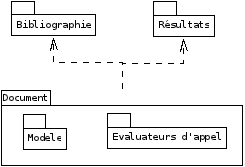
\includegraphics{figures/diagramme-paquetage.png}}
    \caption{Découpage en paquetages du prototype}
    \label{paquetages}
\end{figure}
\begin{itemize}
    \item Document - contient le modèle et les évaluateurs d'appel;
    \item Bibliographie - contient ce qui a trait à l'extraction des métadonnées des citations et l'acquisition de ressources en ligne;
    \item Résultats - classes pour analyser les résultats des évaluateurs d'appels. 
\end{itemize}

\subsubsection{Diagramme de classe du modèle}
Le diagramme de classe du modèle est présenté à la page~\ref{classesmodele}. En python, les méthodes de classe prennent comme premier paramètre l'instance sur laquelle elles s'appliquent. Ce paramètre est le premier paramètre qui est passé à la méthode et est généralement nommé \emph{self}. Il a été omis du diagramme pour améliorer la lisibilité.

Les classes du modèle sont liées par une relation de composition allant du général au particulier. Les classes les plus générales encapsulent les classes les plus particulières et calculent des statistiques à leur égard.

\begin{figure}
    \centerline{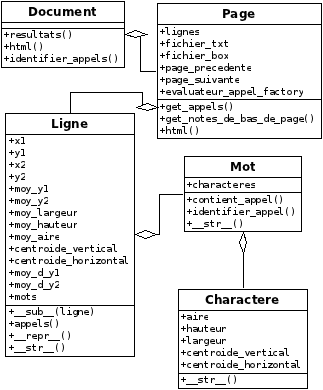
\includegraphics{figures/diagramme-classe-modele.png}}
    \caption{Diagramme de classes du modele}
    \label{classesmodele}
\end{figure}

\subsubsection{Diagramme de classe du module résultats}
Le module résultats contient deux classes: FichierRésultats et ComparateurResultats. FichierRésultats encapsule un \emph{parser} XML qui lit un fichier de résultats d'identification d'appels. \footnote{Le format de ce fichier est présenté dans la section \emph{Identification des appels}}. La méthode eq est implémentée pour surcharger l'opérateur "=": fichier1 = fichier2 retournera vrai si les deux ont identifié les mêmes appels dans les mêmes pages

La méthode compare initialise un ComparateurResultats à partir du résultat entre les deux fichiers. Le FichierRésultats sur lequel la méthode est appelée sera considéré comme la référence. Le diagramme de classes est présenté à la page~\ref{classesresultat}

\subsubsection{Diagramme de classe du module Evaluateurs d'appels}
L'implémentation du module d'évaluation d'appels repose sur le patron \emph{composite} et le patron \emph{factory} tels qu'identifiés par Gamma et \emph{al.} dans \emph{Design patterns}\cite{gamma1995design}. Une interface nommée \emph{EvaluateurAppel} spécifie que les évaluateurs d'appels devront implémenter une méthode \emph{isappel} prenant comme paramètre un caractère et dire si ce caractère est un appel de note de bas de page ou non; une série d'évaluateurs concrets encapsulant chacun une règle précise ont été implémentés. La classe \emph{EvaluateurComposite} est un évaluateur spécial qui contient plusieurs évaluateurs spécifiques et qui retourne "Vrai" si et seulement si tous ses évaluateurs retournent Vrai, ce qui permet de représenter des règles d'identifications complexes. En outre, il est possible de représenter diverses granularités de règles étant donné qu'un \emph{EvaluateurComposite} peut être encapsulé par un \emph{EvaluateurComposite} à son tour. La seule classe à être couplée à tous les évaluateurs concrets est la classe EvaluateurAppelFactory: celle-ci connaît les règles qui régissent l'identification des appels et peut créer un EvaluateurAppelComposite pour une page précise.

La logique spécifique des évaluateurs d'appels est décrite à la page~\pageref{tableau-evaluateurs}. Le diagramme de classe est présenté à la page~\pageref{classesresultat}
\begin{figure}
    \centerline{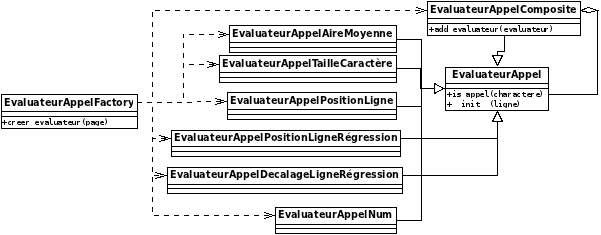
\includegraphics{figures/diagramme-classe-evaluateurs.png}}
    \caption{Diagramme de classes du module «Évaluateurs d'appels»}
    \label{classesevaluateurs}
\end{figure}


\begin{figure}
    \centerline{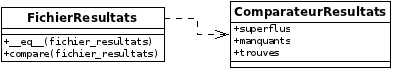
\includegraphics{figures/diagramme-classe-resultats.png}}
    \caption{Diagramme de classes du module résultats}
    \label{classesresultat}
\end{figure}


%\indent Les différentes architectures qui placent les services réseau au centre des décisions ont été rejetées car elles ne sont pas adaptées au présent problème. Deux styles d'architectures ont été évalués plus en détail: l'architecture en couches et l'architecture de type \emph{Pipes and Filters}.

%Dans une architecture en couches, chaque couche supplémentaire correspond à un degré d'abstraction plus élevé. Chacune des couches a une cohérence interne qui correspond à son degré d'abstraction du problème et est isolée des autres couches. L'interface de communication entre les différentes couches en est une de consommation de services, où chacune des couches fournit des services à sa couche supérieure. De bons exemples d'implémentation de cette architecture sont les modèles OSI et TCP/IP.

%Un exemple d'architecture en couche qui pourrait résoudre le problème est présenté dans la figure \ref{f1}. L'utilisateur utiliserait une interface graphique pour lancer une commande permettant de créer un document PDF à partir d'une image. Cette commande ferait appel à la couche «Construction de PDF» sachant que celle-ci fournit le service. Puisque la conversion d'une image en PDF passe par l'étape intermédiaire d'une conversion en LaTeX, la couche «Construction du document LaTeX» serait appellée pour fournir le service. Cette couche coordonnerait alors les appels vers les différents services de la couche inférieure, à savoir la reconnaissance de caractères, l'extraction de méta-données et l'acquisition des ressources bibliographiques. Enfin, ce serait le service de reconnaissance de caractères qui utiliserait la couche pré-traitement afin de faire les traitements nécessaires pour augmenter la précision de la reconnaissance de caractères (augmentation du contraste, alignement des colonnes, etc.). La couche « Numérisation » est déconnectée puisqu'elle est en quelque sorte optionnelle dans ce modèle, mais on pourrait concevoir que l'utilisateur puisse vouloir accéder à une fonction de type « Numériser un document».

%L'architecture \emph{Pipes and Filters} correspond à la métaphore d'un pipeline dans lequel l'information circulerait: le chemin est fixé et lorsque l'information a circulé, il n'y a pas de retour en arrière possible. Dans ce modèle, les filtres sont les logiciels qui modifient l'information et le pipeline est le canal de communication entre eux. La terminologie est en ce sens la même que celle des systèmes UNIX où ce type d'architecture est utilisé pour les commandes système. À titre d'exemple, on peut mentionner \emph{sed} et \emph{awk}.

%Dans notre cas, l'application de l'architecture \emph{Pipes and Filters} impliquerait que le problème soit décomposé en un ensemble de filtres ayant chacun une cohésion assez grande pour pouvoir être utilisé individuellement. Un exemple est proposé dans la Figure \ref{f2}. Deux processus ont été identifiés: le premier concerne l'extraction des méta-données et le deuxième concerne l'insertion des liens vers les ressources dans le document. Ils ont été séparés car l'insertion des hyperliens dans les documents est facultative et qu'il est difficile d'estimer le temps pour faire la recherche.

%Chacune de ces architecture a ses avantages. Dans une architecture en couches la solution est considérée comme un tout, tandis qu'avec une architecture de type \emph{Pipes and Filters} l'emphase est mise sur les propriétés des différents filtres. Nous estimons qu'il est plus facile de tenir compte des attributs qualité reliés à l'ergonomie et l'expérience utilisateur en ayant une vision holiste de la solution. En revanche, ce problème se prête bien à une architecture de type \emph{Pipes and Filters} puisque les filtres obtenus ont, à l'exception du filtre « Recherche de la ressource » car il dépend de ressources externes, les propriétés suivantes:

%\begin{itemize}
%    \item Sortie conditionnée uniquement par les entrées.
%    \item Aucun état à gérer
%    \item Aucune intervention de l'utilisateur (non-interactif) 
%\end{itemize}
%
%[expliquer pourquoi on conserve P\&F]
%
%Il est à noter cependant que notre modèle ne respecterait pas l'architecture \emph{Pipes and Filters} classique où l'information prend la forme d'un flux qui est \emph{immédiatement} envoyé au filtre suivant. Dans le cas qui nous intéresse, cela impliquerait que les caractères soient envoyés au filtre d'extraction de citations au fur et à mesure qu'ils sont reconnus. Or, il est plutôt nécessaire de considérer la page entière -- voir le chapitre, dans le cas où les citations seraient à la fin -- dans son ensemble pour pouvoir extraire les citations: l'information ne se trouve pas dans chaque caractère, mais plutôt dans la relation entre ceux-ci. Cette entorse au modèle ne devrait cependant pas poser problème dans la mesure où les critères énoncés ci-haut sont respectés.

%   \begin{figure}
%   \centerline{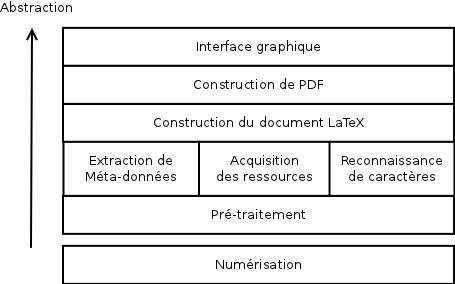
\includegraphics{figures/diagramme-couche.png}}
%    \caption{Exemple d'architecture en couche possible pour résoudre le problème}
%    \label{f1}
%    \end{figure}
%
%   \begin{figure}
%    \centerline{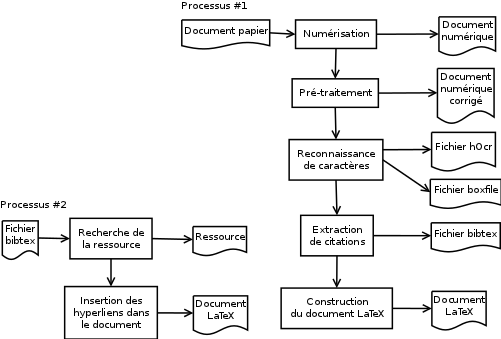
\includegraphics{figures/diagramme-flux.png}}
%    \caption{Exemple d'architecture de type \emph{Pipes and Filters} possible}
%    \label{f2}
%    \end{figure}




\subsection{Reconnaissance de mise en page et de caractère}
Le premier choix a été d'utiliser les logiciels libres \emph{tesseract}~\cite{smith2007overview} et \emph{OCRopus}~\cite{breuel2008ocropus}. Ils ont été choisis car ils sont les références parmi les logiciels d'OCR publiés sous forme de logiciels libres et que la nature de ce projet ne justifie pas l'achat d'un produit commercial
.
OCRopus est un système d'analyse de document et de reconnaissance de caractère modulaire. Plusieurs scripts sont fournis pour faire la reconnaissance de mise en page de document et il est -- théoriquement -- possible d'utiliser différents modules de reconnaissance de caractère, bien que pour le moment un seul module soit fourni. Ce module est \emph{tesseract}, le logiciel de OCR à code source ouvert le plus mature et le plus précis. 

Ocropus décrit la mise en page du document dans le format hOCR. Il s'agit en fait d'un document utilisant les balises HTML standard et auquel a été ajouté un ensemble de classes de style servant à donner de l'information supplémentaire sur la mise en page. Ces fichiers peuvent donc être lus par tout navigateur et la mise en page peut être transformée avec des feuilles de style CSS. Un exemple de fichier produit par OCRopus est présenté à la page~\pageref{sortie-ocropus}.

À partir d'une image d'entrée, Tesseract peut produire deux types de fichiers: un fichier texte et un fichier de type \emph{boxfile}. Le fichier texte contient tous les caractères qui ont été reconnus par le logiciel, sans aucun formatage.

Le fichier \emph{boxfile} est le fichier qui est utilisé pour entraîner tesseract à reconnaître de nouvelles langues. Il consiste en une série de ligne contenant chacune un caractère reconnu et les dimensions de la boîte faisant le contour de se caractère. Un exemple est présenté à la page~\pageref{sortie-tesseract}.

\fontsize{3.5mm}{4.5mm}\selectfont
\lstset{language=python}

\begin{figure*}
\begin{lstlisting}
G 8 117 44 151 0
r 46 117 65 140 0
o 66 117 90 141 0
u 92 117 120 140 0
p 121 105 149 140 0
e 153 117 174 140 0
d 202 117 228 152 0
' 232 134 240 151 0
\end{lstlisting}
\label{sortie-tesseract}
\caption{Exemple de fichier boxfile produit par tesseract}
\end{figure*}
\fontsize{4.5mm}{6.5mm}\selectfont
\begin{figure*}
\fontsize{3.5mm}{4.5mm}\selectfont
\lstset{inputencoding=utf8/latin1}
\lstinputlisting[language=html]{code/giep-logo.html}
\fontsize{4.5mm}{6.5mm}\selectfont
\caption{Exemple de sortie OCRopus}
\label{sortie-ocropus}
\end{figure*}

L'utilisation de OCRopus a finalement été rejetée pour de multiples raisons:
\begin{enumerate}
    \item Tesseract donne des résultats moins précis lorsqu'il est utilisé par OCRopus. Il est conçu pour travailler sur un seul caractère à la fois, mais OCRopus l'utilise pour travailler sur un segment de ligne complet;
    \item Le support pour la langue française est absent lorsqu'on utilise Tesseract via OCRopus. Cela contribue à diminuer la précision de la reconnaissance faite par tesseract.
    \item La documentation d'OCRopus est défaillante. Le code vient avec bon nombre de scripts de reconnaissance mais certains ne sont pas vraiment utilisables.
\end{enumerate}

Pour le prototype, les fonctionnalités intéressantes de OCRopus, c'est-à-dire l'information sur les coordonnées des lignes, ont pu être réimplémentées sans trop d'effort. 

L'utilisation d'OCRopus aurait pu s'avérer plus avantageuse à long terme, et plus particulièrement pour le traitement de documents avec une mise en page complexe. Il faut rappeler que tesseract reconnaît les caractères, mais ignore complètement la mise en page du document, ce qui peut devenir une limitation dans le cas des documents ayant une mise en page complexe.


\subsection{Extraction de citations}
L'extraction de citations consiste à reconnaître les citations pour en extraire les métadonnées. Le problème a été décomposé en trois parties: la reconnaissance de l'appel, la reconnaissance de la citation et l'extraction des métadonnées contenues dans la citation.

\subsubsection{Identification de l'appel}
Les propriétés de l'appel sont relativement homogènes d'un document à l'autre. Il s'agit généralement d'un chiffre placé en indice dont la taille de police est plus petite que celle du reste du texte. Certains éditeurs distinguent les notes du traducteur de celles de l'auteur en utilisant des lettres à la place des chiffres, mais ce n'était pas le cas pour le document utilisé pour concevoir le prototype.

Le prototype a été conçu selon l'hypothèse que toutes les règles de présentation pouvaient être connues \emph{a priori} et qu'il était par conséquent possible d'implémenter une solution sous la forme d'un système expert. L'avantage de cette solution est sa simplicité d'implémentation.

\subsubsection{Évaluation de la méthode}

La combinaison finale d'évaluateurs d'appels a été trouvée de manière itérative en formulant une nouvelle hypothèse à chaque étape. Un protocole d'évaluation de la méthode a été mis en place afin d'évaluer les performances des différentes combinaisons d'évaluateurs d'appel et ainsi valider ou infirmer l'hypothèse posée. Les mesures utilisées pour évaluer les performances des identificateurs d'appels ont été le taux de rappel et le taux de précision.

Le taux de rappel correspond au ratio du nombre d'éléments correctement identifiés à une classe sur le nombre total d'éléments de cette classe; le taux de précision correspond au ratio du nombre d'éléments correctement identifiés à une classe sur le nombre total d'éléments identifiés à cette classe.

Dans un premier temps, un fichier de correctif a été créé. Il s'agit d'un fichier XML contenant l'ensemble des appels pouvant être potentiellement identifiés, c'est-à-dire uniquement ceux dont le chiffre d'appel a été correctement identifié par tesseract, présenté dans le format suivant:

\begin{lstlisting}
<document>
    <page>
        <titre>./tests/revuesociete01-003t</titre>
        <appel>
            <indice>1</indice>
            <terme>sujet</indice>
        </appel>
    </page>
    ...

    ...
</document>
\end{lstlisting}

Lorsqu'il est exécuté, le logiciel produit un fichier qui est dans le même format que le fichier contenant le correctif. Ce fichier peut ensuite comparer ce fichier à celui produit par le logiciel de la manière suivante:

\begin{lstlisting}
$ python citations.py --comparaison correctif.xml resultats.xml resultats-comparaison.xml
\end{lstlisting}

Dans cet exemple, resultats-comparaison.xml est le fichier obtenu par la comparaison de correctif.xml et de resultats.xml et il compte quatre sections: les résultats (rappel et précision) ainsi que les sections \emph{trouves}, \emph{manquants} et \emph{superflus}.

La section \emph{Trouvé} correspond aux appels identifiés correctement; \emph{manquantes} correspond aux appels présents dans le correctif et manquants dans les résultats, tandis que \emph{superflus} représente l'inverse.

Le rappel et la précision sont calculés comme suit:
\[
rappel = \frac{\|trouves\|}{\|total\|}
\textrm{  et  } 
précision = \frac{\|trouves\|}{\|trouves + superflus\|}
\]

\begin{table}
\begin{tabular}{| p{4cm} | p{12cm} |}
    \hline
    \rowcolor[gray]{0.9}
    EvaluateurAppel & Description \\
    \hline
    EvaluateurAppelPosition\linebreak Ligne & Détermine si un caractère est utilisé comme appel à partir de l'écart entre son centroïde vertical et le centroïde vertical de la ligne. Le centroïde vertical de la ligne est calculé à partir de la moyenne des positions y1 et y2 de chacun des caractères contenus dans celle-ci. Un caractère est identifié comme un appel si son centroïde vertical est plus haut que celui de la ligne. Cette méthode est rapide, mais elle est inefficace dans le cas où le document a été numérisé avec un biais et que la ligne n'est pas droite. Pour un exemple d'erreur voir~\ref{erreur-evaluateurpositionligne} \\
    \hline
    EvaluateurAppelTaille\linebreak Caractere & Détermine si un caractère est un appel en comparant son aire à l'aire moyenne des caractères de la même ligne. Le caractère est indentifié comme étant un appel si le rapport de son aire sur l'aire moyenne est en-deça d'un certain seuil spécifié par l'utilisateur. \\
    \hline
    EvaluateurAppelPosition\linebreak LigneRegression & Même principe que \emph{EvaluateurAppelPositionLigne}. Cependant, plutôt que de vérifier si le centroïde vertical du caractère est plus haut que le centroïde vertical de la ligne, on vérifie si le centroïde vertical du caractère est plus haut que la droite de régression calculée en utilisant les centroïdes horizontaux et verticaux des caractères de la ligne. Plus lent, mais plus efficace dans les cas où le document est numérisé avec un biais. \\
    \hline
    EvaluateurAppelAlphaNum & Un caractère est un appel s'il est alpha-numérique. \\
    \hline
    EvaluateurAppel\linebreak Numerique & Un caractère est un appel s'il est numérique \\
    \hline
    EvaluateurAppelDecalage\linebreak LigneRegression & Un caractère est identifié comme un appel s'il est en décalage avec la ligne. Le décalage est calculé en utilisant les positions y1 et y2 du caractère et en les comparant avec les deux droites de régression passant par les positions y1 et y2 des caractères de la ligne. \\
    \hline
\end{tabular}
\begin{figure*}
\centerline{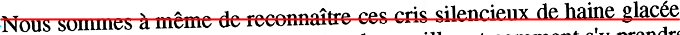
\includegraphics{figures/exemple-ligne-decalee.png}}
\caption{Exemple d'erreur que fait l'EvaluateurPositionligne lorsque les lignes sont décalées}{Dans cette image, la ligne rouge représente le centroide vertical, qui est calculé pour être entre les y1 moyen et les y2 moyen de la ligne. Vu que la ligne est décalée, certaines lettres se trouvent à être plus haut que le centroïde vertical et sont alors considérées comme des appels}
\label{erreur-evaluateurpositionligne}
\end{figure*}
\label{tableau-evaluateurs}
\caption{Évaluateurs d'appels utilisés dans le prototype}
\end{table}
L'ensemble d'évaluateurs le plus simple qui soit a été utilisé dans un premier temps pour obtenir les valeurs sur lesquelles se baser pour optimiser la solution. Les combinaisons utilisées pour le prototype sont présentées à la page~\pageref{combinaisons-evaluateurs}.
\begin{table}
\begin{tabular}{| p{6cm} | p{2cm} | p{1.25cm} | p{6cm} |}
    \hline
    \rowcolor[gray]{0.9}
    Evaluateurs & Précision & Rappel & Observations et hypothèses \\
    EvaluateurAppelPositionLigne, EvaluateurAppelAlphaNum et EvaluateurAppelTaile (Seuil = 0.6)
    & $0.30$ & $0.28$ & 
    \begin{itemize}
        \item Les appels non numériques peuvent être enlevés (il y en a aucun dans le texte)
        \item Beaucoup d'erreurs dans les pages dont la numérisation est mal alignée. Peut-être dû au fait que l'algorithme ne tient pas compte de ce décalage en calculant les 
        \item Certaines erreurs sont dûes au fait que l'évaluateur trouve uniquement un appel (sans terme qui le porte).
        \end{itemize}  \\ \hline
        EvaluateurAppelPositionLigne,
        EvaluateurAppelNumerique et 
        EvaluateurAppelTaille (Seuil = 0.6)
    & $1.0$ & $0.37$ &
    \begin{itemize}
        \item Précision augmentée à 100\% depuis que seuls les chiffres sont considérés comme des appels.
        \item Tester l'evaluateur d'appel de régression linéaire.
    \end{itemize} \\
    \hline
        EvaluateurAppelPositionLigne (régression linéaire),
        EvaluateurAppelNumerique et
        EvaluateurAppelTaille (Seuil = 0.6)
    & $1.0$ & $0.37$ &
    \begin{itemize}
        \item Aucune amélioration depuis que la position par rapport à la ligne est calculée avec une droite de régression linéaire. 
        \item La majorité des erreurs sont dûes à un changement de notation de l'appel. 
    \end{itemize}
        \\ \hline
    EvaluateurAppelPositionLigne, EvaluateurAppelNumerique et EvaluateurAppelTaille pour la première partie. EvaluateurAppelDecalage, EvaluateurAppelNumerique et EvaluateurAppelTaille pour la deuxième partie &
    $0.78$ & $0.86$ &
    Baisse de la précision dûe au fait que les références à une page sur une ligne où il n'y a pas beaucoup de texte (ex: "p. 88") sont identifiés comme des appels puisque les chiffres sont plus haut que le caractère (donc décalés).
    \\ \hline
    \emph{idem.} & $0.82$ & $1.0$ &
    Amélioré le rappel en enlevant l'ÉvaluateurAppelTaille de la deuxième section. Amélioré la précision en ajoutant une règle qui agit au niveau du mot pour éliminer les cas où une référence à un numéro de page est interprété comme étant un appel.
    \\ \hline
\end{tabular}
\caption{Combinaisons d'évaluateurs d'appel utilisés dans le prototype}
\label{combinaisons-evaluateurs}
\end{table}

\subsubsection{Problèmes rencontrés et améliorations possibles}
Le problème principal a été dû à la qualité de la reconnaissance de caractères faite par tesseract. Bien que les résultats obtenus soient de manière générale satisfaisants, la reconnaissance des caractères d'appel s'est avérée très imprécise. En effet, dans la première partie, où les caractères d'appel étaient caractérisés par une plus petite taille et une position en appel, ces derniers ont la plupart du temps été confondus avec des caractères de ponctuation divers, par exemple l'apostrophe ou l'accent circonflexe.

Une configuration générique de tesseract a été utilisée pour faire la reconnaissance: les fichiers de langue française fournis avec la distribution \emph{Arch Linux}. Il serait possible d'améliorer la configuration de tesseract par une ou plusieurs des manières suivantes:
\begin{itemize}
    \item En entraînant tesseract pour la police particulière utilisée dans le document;
    \item En fournissant une liste de mots courants dans le document lors du lancement de tesseract. Cette liste de mots aide à préciser la numérisation en représentant plus fidèlement le modèle du texte numérisé;
    \item En fournissant une liste "DangAmbigs" comprenant les ambiguïtés couramment rencontrées dans le texte. Ce fichier contient les principaux de substitution dans une langue. Un exemple est fourni à la page~\pageref{figure-dangambigs}.
\end{itemize}

Entraîner tesseract en utilisant ces méthodes aurait pris du temps et aurait débordé du cadre du projet. Le fichier texte a plutôt été corrigé à la main, autant dans le fichier texte que dans le fichier \emph{boxfile}, lorsque c'était facile -- c'est-à-dire dans les cas autres que ceux où une lettre a été représentée par deux lettres (exemple h -> l n).

\begin{figure*}
\begin{lstlisting}
1	m	2	r n
2	r n	1	m
1	m	2	i n
2	i n	1	m
1	d	2	c l
...
...
\end{lstlisting}


\caption{Exemple de fichier DangAmbigs}{La première ligne indique que tesseract peut confondre un caractère (le m) pour deux caractères (r et n). La ligne suivante décrit le cas inverse, où deux caractères (r et n) sont confondus avec le m}
\label{figure-dangambigs}
\end{figure*}
Une autre limitation est due à l'implémentation de la solution. Les évaluateurs d'appel ont été implémentés pour évaluer une seule lettre à la fois et pour être initialisés à partir d'une ligne. Or, il serait préférable que ceux-ci puissent évaluer un mot au complet et être initialisés à partir du document au complet. Cette amélioration de conception aurait été utile pour certains évaluateurs, notamment celui détermine si un caractère est un appel à partir du ratio de la taille du caractère sur la taille moyenne des caractères d'une ligne. En l'entraînant à partir d'une seule ligne, il n'y a pas assez d'occurrences d'un même caractère de disponibles pour que ce soit une base de comparaison valide. La taille du caractère doit alors être comparée à la taille moyenne des autres caractères de la ligne nonobstant le contenu précis du caractère. Cela a comme effet que les caractères de ponctuation sont systématiquement perçus comme des appels, bien qu'en réalité ils ne le soient pas.



\subsubsection{Extraction des métadonnées}
La forme que prennent les citations dans le texte est déterminée selon une convention. Mais au-delà du fait que la convention invite l'auteur à fournir toutes les informations pertinentes qui pourraient aider le lecteur à retracer l'oeuvre citée, elle n'oblige à aucun formalisme. Ainsi, le format des références peut varier grandement. La figure~\ref{f4} montre les quelques premières citations de notre échantillon.

\fontsize{3.5mm}{4.5mm}\selectfont
\begin{table}
\begin{tabular}{| p{8cm} | p{8cm} | }
    \hline
    \rowcolor[gray]{0.9}
    Exemple & Format \\
    L'idéologie allemande, Paris, La Pléiade, 1982, p. 1085. & <TITRE>, <VILLE>, <COLLECTION>, <ANNÉE>, p. <PAGE>. \\
    \hline
    "Fini le règne des idéologies, place aux acteurs sociaux, Le Devoir, mercredi le 7 janvier 1987. & "<TITRE>, <PUBLICATION>, <DATE>. \\
    \hline
    \multicolumn{2}{|l|}{Note: le guillemet anglais manquant est dans le texte.} \\ 
    \hline
    Voir ici le texte de Alain Caillé & Voir <PUBLICATION> le texte de <AUTEUR> \\
    \hline
    Nicole Gagnon, La réforme scolaire au Québec, Université Laval, 1986 & <AUTEUR>, <TITRE>, <ÉDITEUR>, <ANNÉE> \\
    \hline
    Ou encore: "At last count, 50 percent of the American population believed an accused individual guilty until proven innocent; 50 percent didn't know which side the United States support in Nicaragua; 42 percent couldn't name an asian country "near the pacific ocean"; and 40 percent of the nation's High School seniors thought that Israel was an arab country". Lewis H. Lapham, Harper's Magazine, september 1987, p. 8. & <NOTE>, <AUTEUR>, <PUBLICATION>, <DATE>, <PAGE> \\
    \hline
    Les emplois en 1990: les options gagnantes, Ministère de l'Éducation, cité par Paul Bernard, "Imaginer le réel pour réaliser l'imaginaire", La sociologie et l'anthropologie au Québec, Cahiers de l'ACFAS, 1985, p. 112. & <TITRE-ORIGINAL>, <ÉDITEUR-ORIGINAL>, cité par <AUTEUR>, <TITRE-TEXTE>, <TITRE>, <ÉDITEUR>, <ANNÉE>, p. <PAGE>. \\
    \hline
    \multicolumn{2}{|l|}{Note: le guillemet anglais manquant est dans le texte.} \\ 
    \hline
\end{tabular}

\caption{Exemples de citations trouvées dans le texte}
\label{f4}
\end{table}
\fontsize{4.5mm}{6.5mm}\selectfont
Selon Afzal \emph{et coll.} \cite{afzal2009improving}, cette variation de la forme de la citation est surtout induite par des facteurs humains (les éditeurs ont leur propre style, les auteurs peuvent faire des erreurs dans le titre d'un texte cité, etc.) et est l'un des problèmes majeurs dans la conception d'outils d'extraction de métadonnées.

On peut remarquer dans les exemples ci-dessus que le formalisme des citations les situe à mi-chemin entre un langage formellement codifié et le langage naturel. Plutôt qu'un ensemble de règles formelles, il s'agit de conventions (suivies à un degré plus ou moins grand dépendant des disciplines) qui ont été élaborées par des humains afin d'échanger de l'information. Il n'existe pas, au final, d'ensemble fermé de règles permettant de reconnaître l'ensemble des citations possibles.

Cette avenue a tout de même été testée en tentant de créer un ensemble exhaustif d'expressions régulières. L'hypothèse portée par cette solution est que les expressions régulières peuvent être classées par ordre de restrictivité. Ainsi, la première à être testée est celle qui permet de récupérer le plus de champs (par exemple: Nom, Prénom, Titre, Maison d'édition, Collection, Ville, Année, pages) et la dernière à être testée est celle qui récupère le moins de champs (par exemple: Nom, Titre, Année). Ainsi, si l'une des expressions régulières de l'ensemble est en mesure de retourner de l'information, on peut prendre pour acquis qu'il m'aurait pas été possible d'obtenir plus d'information autrement.

Le problème qui se pose rapidement est celui du critère d'ordonnancement. Comment peut-on distinguer le format "<Auteur>, <titre>, <collection>, <annee>" du format "<Auteur>, <titre>, <editeur>, <annee>", ou encore du format "<titre>. <Auteur>, <editeur>"? Ces champs ne sont pas caractérisés par un format quelconque qu'il serait possible de reconnaître avec une expression régulière. Au regard d'une expression régulière, les différents champs sont équivalents puisque les expressions régulières sont incapables de saisir leur contenu sémantique.

Les différentes manières d'exprimer les citations sont infinies, mais l'ensemble de règles qui les évaluera sera toujours fini. En créant les règles, on se rend rapidement compte que celles-ci doivent toujours être adaptées aux spécificités du domaine. 

Le choix final a plutôt été d'utiliser une librairie implémentée en \emph{ruby} et distribuée sur le site \emph{github} en logiciel libre. Cette librairie, \emph{anystyle-parser}~\cite{anystyleparser}, implémente des \emph{Conditional Random Fields} pour étiqueter les parties d'une citation. Elle est distribuée avec un ensemble d'entraînement et est donc rapidement utilisables.

Anystyle-parser a de manière générale bien réussi à étiqueter les parties d'un ensemble de citations trouvées sur \emph{Google Scholar}. La plupart des erreurs étaient dans le type d'entrée BibTeX, en confondant \emph{inproceedings} avec \emph{incollection}, par exemple. Par contre, en utilisant \emph{anystyle-arser} tel que distribué, son utilisation dans le contexte de ce projet a été un échec étant donné qu'aucune citation n'a pu être étiquetée convenablement sauf dans un seul cas (celui de la citation de Nicole Gagnon présentée ci-haut).

Ce faible taux de réussite peut être attribué à plusieurs facteurs. Dans un premier cas, il faut noter que le modèle fourni avec anystyle-parser ainsi que tout l'ensemble d'entraînement ont été faits en anglais. Il est donc normal que, si entraîné en anglais, le logiciel éprouve des difficultés à généraliser en français.

Les problèmes de généralisation dus à la langue française se font sentir d'autant plus que les notes de bas de page présentes dans le document utilisé sont très souvent écrites en texte libre. Dans les publications du domaine des sciences naturelles, appliquées ou de l'ingénierie, la distinction entre une note de bas de page et une référence bibliographique est plus claire que dans les sciences humaines. En sciences humaines, la référence bibliographique est présentée dans une note de bas de page, mais on ne peut pas réduire une note de bas de page à une référence bibliographique. Il faut prendre pour acquis qu'il y aura du texte avant et après la référence bibliographique: il est donc nécessaire de pouvoir extraire la référence bibliographique de son contexte, ce qu'\emph{anystyle-parser} n'est pas conçu pour faire -- il arrive tant bien que mal à donner des résultats sensés en anglais, mais en français l'étiquetage semble être totalement arbitraire.


\subsection{Génération du document HTML}
Tout au long du projet, le \emph{document} a été le modèle avec lequel nous avons travaillé. Dans le même ordre d'idées, il est facile de considérer le document produit comme étant une vue dans le paradigme \emph{modèle-vue-contrôleur} (MVC). Ainsi, le document devient le modèle abstrait, tandis que la représentation HTML devient la vue qui représente ce document. Le contrôleur pourrait être une classe tierce qui apporterait des modifications au modèle à partir d'information reçue par la vue (si l'on implémente une vue HTML, cette vue pourrait être un ensemble de boîtes de saisie de texte).

Dans cette optique, la mise en page devient l'action d'appliquer une vue précise au modèle de document. Le patron modèle-vue-contrôleur suggère que, pour simplifier l'implémentation et la rendre plus facile à maintenir, il est nécessaire de préserver l'indépendance entre la vue et le modèle. Ainsi, le modèle ne doit pas contenir d'information concernant sa représentation tout comme la vue ne doit pas contenir de code exprimant une logique interne au modèle (par exemple, la vue ne doit pas contenir de code servant à déterminer si une partie du texte est un appel).

Pour notre implémentation du MVC, nous avons utilisé une librairie de gabarits (de \emph{templating} en anglais). Ces librairies sont couramment utilisées dans les implémentations web du patron MVC. En effet, depuis qu'ils ont été popularisés avec \emph{Ruby on Rails}, les templates ont été présents dans toutes les librairies web récentes. En ce qui concerne python, plusieurs librairies sont disponibles, par exemple \emph{Mako} et \emph{Jinja2}. 

La manière de rédiger un gabarit varie très peu d'un système à l'autre. Si les systèmes de gabarit présentent quelques différences du point de vue de la syntaxe, ils reposent tous sur le même principe: les gabarits sont écrits dans un format choisi par l'utilisateur (HTML, LaTeX, Markdown, etc.). Le texte du gabarit n'est pas compilé et l'utilisateur est libre d'écrire ce qu'il veut, à l'exception de certains mots-clé réservés qui permettent de coder une logique de mise en page. Ces mots-clés servent par exemple d'interrroger des variables, de faire des boucles, etc. En outre, le gabarit est produit par l'appel d'une fonction python standard, et les variables auxquels il a accès sont celles qui ont été fournies lors de l'appel de la fonction.

Pour notre système, le choix du système de gabarits n'est pas critique. Ils n'ont pas de grande différence du point de vue de l'implémentation, et leurs différences concernent souvent leur implémentation dans un \emph{framework} web python donné. Étant donné que nos gabarits sont hors ligne (ils sont exécutés au plus une seule fois, pour générer le fichier HTML). Pour le projet, \emph{Jinja2} a été utilisé étant donné qu'il est le plus petit et plus simple à mettre en place, bien qu'il soit réputé plus lent que son concurrent \emph{mako}.\footnote{voir http://stackoverflow.com/questions/1324238/what-is-the-fastest-template-system-for-python}
\begin{figure*}
\begin{lstlisting}
<div class="document">
    
        <span class="ligne">{{ ligne }}</span>
    
</div>

\end{lstlisting}
\caption{Exemple de code Jinja2}{Cet exemple de code Jinja2 présente l'itération d' une liste. Si la variable lignes contenait trois lignes, par exemple, le document HTML résultant contiendrait les trois lignes, chacune entourée de sa balise span}
\end{figure*}
En résumé, l'utilisation d'un système de gabarits permet d'avoir une implémentation simple et concise. Puisque le système de gabarits implémente le patron MVC, il est facile de fournir différentes du même document: chacun de ces formats est considéré comme une vue et est implémentée dans son propre fichier. Dans ce projet, il a été question de la représentation HTML du document, mais il aurait été tout aussi simple de le faire en LaTeX, et il serait possible d'ajouter la sortie LaTeX sans modifier le code du modèle.


\subsection{Acquisition des liens vers les références bibliographiques}
L'objectif premier d'une référence bibliographique est d'aider le lecteur à se procurer une copie de l'ouvrage référencé. La codification de la référence bibliographique est l'abstraction sur laquelle repose le classement. Les clés de classement sont les mêmes d'une bibliothèque à l'autre bien que la disposition physique des livres et des collections peut varier.

Le prototype est capable de trouver une ressource bibliographique sur Google Scholar à partir d'une référence Bibtex. Son implémentation est naïve dans la mesure où le prototype fait la recherche de la même manière dont un être humain la ferait.

\emph{Google Scholar} accepte différents paramètres de recherche. On peut par exemple spécifier \emph{intitle} pour chercher dans le titre ou encore \emph{inauthor} pour chercher parmi les noms d'auteurs. Le prototype créera dans un premier temps l'URL de recherche en traduisant les différents de la référence bibtex dans leur équivalent supporté par \emph{Google Scholar}.

La recherche est ensuite faite en utilisant la librairie \emph{urllib} fournie avec la distribution standard de python~\cite{pythonorg}. Cette librairie se charge essentiellement de lancer le "GET" et de gérer les possibles exceptions. Une fois la page retournée, le prototype extraira le premier résultat en BeautifulSoup~\cite{beautifulsoup}, une librairie XML axée sur l'extraction de contenu dans des fichiers HTML.\footnote{Elle se spécialise dans l'extraction de contenu dans la mesure où elle n'est pas optimisée pour la performance, mais plutôt pour être robuste et être capable de travailler avec un fichier extrêmement mal formatté.}

La librairie a été testée avec l'ensemble de test de \emph{anystyle-parser} et a été capable de récupérer toutes les références.  


\subsection{Discussion}
Le but premier d'un prototype est de vérifier si une hypothèse de développement peut être fructueuse et déterminer s'il est souhaitable de poursuivre dans cette voie. Le prototype qui a été implémenté fonctionne bien, hormis dans le cas où la référence bibliographique est précédée de texte libre, mais nécessiterait encore beaucoup de travail pour devenir un produit fini.

En premier lieu, il faut noter que les différents modules sont fonctionnels lorsqu'ils sont exécutés indépendamment les uns des autres, mais que les défis propres à leur intégration n'ont pas encore été résolus. La raison principale est que l'une des hypothèses de travail s'est avérée être fausse: on ne peut pas dire qu'il y a identité entre une référence bibliographique et une note de bas de page.
L'implémentation de \emph{anystyle-parser} est efficace pour étiqueter les parties de la référence bibliographique, mais est incapable d'identifier une «non-référence»: elle prend pour acquis qu'elle aura une référence complète, ce qui est pratiquement jamais le cas dans le domaine de ce projet. Il devient donc nécessaire d'implémenter une librairie qui fait l'extraction de la référence bibliographique dans un document rédigé en texte libre et qui deviendrait l'étape préalable à l'étiquetage. Cette librairie devra aussi être capable de gérer les références symboliques dans le texte (par exemple l'utilisation de \emph{ibid}, pour référer à la dernière citation, \emph{op cit.}, pour référer au texte cité plus haut, etc.)


La librairie \emph{anystyle-parser} devra ensuite être entraînée pour fonctionner avec des références en français. Il est raisonnable de penser qu'il est possible d'obtenir, avec un modèle correctement entraîné, des résultats similaires à ceux obtenus avec des références bibliographiques en anglais.

Par ailleurs, la performance de \emph{anystyle-parser} est médiocre dans le prototype. L'implémentation du prototype est en python tandis que celle de cette librairie est en ruby: le prototype lance l'interpréteur ruby à chaque fois qu'il doit analyser une référence bibliographique, ce qui prends à chaque fois quelques secondes.

Pour résoudre ce problème, la meilleure solution serait à notre avis d'exécuter la librairie comme un service web et de communiquer avec elle dans un format intermédiaire, par exemple JSON. De cette manière, l'interpréteur ruby ne serait lancé qu'une seule fois. Il s'agit d'une solution pragmatique: il serait par ailleurs moins compliqué d'implémenter ce service web avec un serveur léger comme \emph{Sinatra}~\cite{sinatrarb} que de réimplémenter \emph{anystyle-parser} en python.

Du point de vue de la conception, des modifications doivent être apportées pour finir de découpler les modules. Le modèle, tel qu'implémenté dans le prototype, peut apporter de sérieuses limitations à long terme. Dans le prototype, il y a confusion entre les informations concernant la structure du document (les pages, les mots, etc.) et l'information sémantique (les appels et les références bibliographiques) du document. Les deux niveaux sont implémentés dans les mêmes objets, et les informations sémantiques sont obligatoirement rattachées à un de ces objets du modèle: par exemple, autant l'appel de note de bas de page que la citation doit être rattachée à une page.

Pour faire évoluer le prototype et être capable de travailler avec d'autres systèmes de notation des appels (où les références sont toutes regroupées en fin de chapitre ou en fin de document, par exemple), il serait important de poser cette distinction entre le niveau structurel et le niveau sémantique. Une solution pourrait être d'implémenter un système d'annotation sémantique qui agirait sur un modèle qui serait dépouillé de tout sauf les informations structurales. Le modèle pourrait être réutilisé plus facilement pour d'autres applications -- notamment la simple correction de numérisations.

Le prototype a été conçu pour faire la recherche sur Google Scholar. Il s'acquite bien de cette tâche. Il a cependant été conçu selon l'hypothèse que les bibiliothèques virtuelles seraient similaires. Après vérification, cette hypothèse s'est avérée être fausse: chaque bibliothèque requiert sa propre implémentation. Pour Google Scholar et arXiv, on peut utiliser leur API \emph{ATOM} pour accéder aux ressources. Certaines bibliothèques n'offrent pas ces ressources et on doit alors faire du \emph{screen scraping}\footnote{Ou en français « Capture de données d'écran». Il s'agit de récupérer les informations qui sont destinées au navigateur web.}.


\subsection{Conclusion}
À la suite de la réalisation du prototype, il est permis de conclure qu'il serait possible de poursuivre dans cette voie et de compléter le produit. Bien que certaines modifications soient requises pour passer du stade de prototype au stade de produit fini, la base sur laquelle a été fondé le prototype.

Plusieurs hypothèses ont été posées: certaines ont été confirmées tandis que certaines ont été infirmées. D'abord, il est possible de construire un système expert pour faire l'identification des appels de notes de bas de page. Les règles sont connues \emph{a priori} et il est possible de les codifier: il faut simplement un modèle flexible qui est capable de fournir l'information nécessaire (par exemple la taille moyenne d'une lettre précise du texte)

Il est par contre impossible de présumer que les références bibliographiques citées dans le texte peuvent être identifiées «naïvement» en utilisant des expressions régulières.

En outre, si l'application que nous avons retenue pour le développement du prototype a été l'extraction de ressources bibliographiques, il faut noter qu'il en existe d'autres qui pourraient être intéressantes à explorer. Plus précisément, il serait possible d'utiliser le modèle et le module d'identification de références bibliographiques pour étudier les réseaux au sein des publications académiques en établissant une cartographie des citations. Une fois les citations identifiées et étiquetées, il est possible de construire un index de références et d'établir ainsi les liens entre les publications.


\section*{Annexe A: Plan de travail révisé}
%\fontsize{3.5mm}{3.5mm}\selectfont
\begin{table}
\begin{tabular}{| p{.5cm} | p{2cm} | p{2cm} | p{1.2cm} | p{1.5cm} | p{3.5cm} | p{3.5cm} |}
    \hline
    \rowcolor[gray]{0.9}
    \# & Commencé & Terminé & Effort estimés & Efforts actuels & Tâches & Livrable(s) \\
     \hline 
     1 & 25 oct 2011 & 25 oct 2011 & 1h & .5h & Remise de la fiche de renseignements & Fiche de renseignements \\
     \hline
     2 & 2 oct 2011 & 2 oct 2011 & .5h & .5h & Description du projet / discussion avec professeur superviseur &  \\
     \hline
     3 & 10 oct 2011 & 10 oct 2011 & 10h & 5h & Remise de la proposition de projet & Proposition de projet  \\
     \hline
     4 & 7 oct 2011 & 14 oct 2011 & 10h & 20h & Analyse des outils d'entraînement pour tesseract et OCRopus. Programmation d'une interface d'entraînement pour Tesseract & Code source \\
     \hline
     5 & 15 oct 2011 & 15 oct 2011 & 1h & 1.5h & Rencontre avec C. Desrosiers & \\
     \hline
     6 & 20 oct 2011 & 27 oct 2011 & 5h & 10h & Rédaction du rapport d'étape & Rapport d'étape \\
     \hline
     7 & 20 oct 2011 & 21 oct 2011 & 4h & 8h & Élaboration et comparaison de deux architectures possibles pour résoudre le problème & Rapport final, section « Implémentation » \\
     \hline
     8 & 15 oct. 2011 & 15 oct. 2011 & .5h & 4h & Configuration de l'environnement de développement -- installation/compilation d'OCRopus & \\
    \hline
     9 & & & 15h & & Implémentation du composant d'analyse de document et d'identification de références & Code source \\
    \hline
    10 & & & 20h & & Implémentation du composant de conversion de \emph{hOcr} en LaTeX & Code source \\
    \hline
    11 & & & 1h & & Rencontre de suivi avec C. Desrosiers &  \\
    \hline
    12 & & & 5h & & Prototypage de l'accès à Google Books & Code source \\
    \hline
    13 & & & 15h & & Implémentation du module d'accès aux références & Code Source \\
    \hline
    14 & & & 10h & & Rédaction de la section \emph{Implémentation} du rapport final & Rapport final \\
    \hline
    15 & & & 5h & & Conversion des références en format BibTex & Code source \\ 
    \hline
    16 & & & 10h & & Rédaction des autres sections du rapport final & Rapport final \\
    \hline
    17 & & & .5h & & Présentation du projet & \\
    \hline
\end{tabular}
\caption{Plan de travail}
\end{table}
\bibliographystyle{plain}
\nocite{rubylang}
\nocite{jinja2}
\nocite{makotemplates}
\nocite{pybtex}
\bibliography{biblio}
\end{document}
